\documentclass[conference]{IEEEtran}

%\usepackage{cite}

\usepackage[cmex10]{amsmath}

\usepackage{algorithm}
\usepackage{algorithmic}

% Graph package
\ifx\pdfoutput\undefined
\usepackage{graphicx}
\else
\usepackage[pdftex]{graphicx}
\fi
\usepackage{epstopdf}

\usepackage{multirow}



% *** SUBFIGURE PACKAGES ***
\usepackage[tight,footnotesize]{subfigure}
% subfigure.sty was written by Steven Douglas Cochran. This package makes it
% easy to put subfigures in your figures. e.g., "Figure 1a and 1b". For IEEE
% work, it is a good idea to load it with the tight package option to reduce
% the amount of white space around the subfigures.


%\usepackage[caption=false]{caption}
%\usepackage[font=footnotesize]{subfig}
% subfig.sty, also written by Steven Douglas Cochran, is the modern
% replacement for subfigure.sty. However, subfig.sty requires and
% automatically loads Axel Sommerfeldt's caption.sty which will override
% IEEEtran.cls handling of captions and this will result in nonIEEE style
% figure/table captions. To prevent this problem, be sure and preload
% caption.sty with its "caption=false" package option. This is will preserve
% IEEEtran.cls handing of captions. Version 1.3 (2005/06/28) and later 
% (recommended due to many improvements over 1.2) of subfig.sty supports
% the caption=false option directly:
\usepackage[caption=false,font=footnotesize]{subfig}








% correct bad hyphenation here
\hyphenation{op-tical net-works semi-conduc-tor}


\begin{document}

% can use linebreaks \\ within to get better formatting as desired
\title{Efficient FPGA Implementation of\\ Overclocking Friendly Online Arithmetic Operators}


% author names and affiliations
%\author{\IEEEauthorblockN{Kan Shi, David Boland, and George A. Constantinides}
%\IEEEauthorblockA{Department of Electrical and Electronic Engineering\\
%Imperial College London\\London, UK\\
%\{k.shi11, david.boland03,g.constantinides\}@imperial.ac.uk}
%}

\maketitle


\begin{abstract}
%\boldmath
The abstract goes here.
\end{abstract}


% For peer review papers, you can put extra information on the cover
% page as needed:
% \ifCLASSOPTIONpeerreview
% \begin{center} \bfseries EDICS Category: 3-BBND \end{center}
% \fi
%
% For peerreview papers, this IEEEtran command inserts a page break and
% creates the second title. It will be ignored for other modes.
\IEEEpeerreviewmaketitle



\section{Introduction}

\section{Background and Relevant Work}
\subsection{Online Arithmetic}

%\subsection{FPGA Architecture}


\section{Digit-parallel Online Adder on FPGAs}
\subsection{Related Works}
There has been previous works focusing on efficient FPGA implementation of the digit-parallel online adder. Generally the existing approaches can be classified into three types:%, as discussed below. A more detailed review of current works can be found in xxx.
\begin{enumerate}
	\item efficient mapping of the digit-parallel online adder onto sophisticated FPGAs resources [xxx];
	\item multiple operands addition by designing compressor trees based on bit counters [xxx];
	\item modifying existing FPGA architecture for more efficient online addition [xxx] and for specific applications [xxx].
\end{enumerate}

Type 2 and type 3 are beyond the scope of this paper, as we focus on the general purpose online adder that takes 2 inputs and generate 1 outputs, as shown in Figure xxx. Specifically in type 1, both works took advantage of the built-in carry resources in FPGAs. Conventionally the ASIC implementation of online adders is based on the 4:2 compressors, as shown within the gray background in Figure xxx. However, directly applying this approach in the FPGAs could be less efficient. This is because there is no carry propagation between the 2 full adders within a 4:2 compressor, and the net delay between them can be large. Instead, Kamp et al and Ortiz et al described very similar mapping techniques for online adders with 2 different data representations, respectively. The main idea is to map the logic block within the dotted circle in Fig.~\ref{Fig:PreviousWork}. In this case, the fast-carry logic in the FPGA can be employed, and the delay between the 2 FAs is largely reduced. 

\begin{figure}[htbp]
	\centering
	\includegraphics[width=.5\textwidth]{./Figures/SDAdder_42comp_Spartan.pdf}
	\caption{Map the online adder onto Spartan FPGAs using the fast-carry resources. The grey background highlights the 4:2 compressor. Dotted circle indicates the logic block (LB) which can be mapped to the FPGA carry resources.}
	\label{Fig:PreviousWork}
\end{figure}

However, we notice the major limitations of both approaches that they only target on FPGAs with 4-input LUTs and 2 LUTs within a logic slice, such as the Xilinx Spartan series and the Altera Cyclone series. This is naturally reasonable because one LB can be mapped to a single slice. Nevertheless, for FPGAs with 6-input LUTs (6-LUT) and 4 LUTs in a slice, such as the Xilinx Virtex series and all Xilinx 7 series FPGAs, directly applying the approaches in [xxx] will result in either resource waste or logic fault. For instance, if 2 LBs are mapped to a slice with 4 LUTs as seen in Fig.~\ref{Fig:PreWorkVirtex6}s, the outputs of the second LB will be faulty because the its carry input cannot be explicitly initialized. 

\begin{figure}[htbp]
	\centering
	\includegraphics[width=.45\textwidth]{./Figures/SDadder_FastCarry_PreviousWork.pdf}
	\caption{Direct utilization of previous approaches on a Virtex-6 FPGA will results in faulty outputs.}
	\label{Fig:PreWorkVirtex6}
\end{figure}

\subsection{Proposed Mapping Method} 
To tackle this problem, we first modify the structure of the online adder to enable an efficient FPGA mapping. The structure of a 3-digit online adder is given as an example in Fig.~\ref{Fig:ModifiedOA}. In this equivalent structure, the first FA in each 4:2 compressor is split into 2 parts, which only generate carry and sum respectively. In this case they can be mapped individually on 2 LUTs. The second FA, which generates the outputs, is unchanged and can be implemented using the fast-carry logic.


%propose an alternative mapping method that targets on the slice containing 4 LUTs such as the Xilinx Virtex series and all Xilinx 7 series FPGAs. 

\begin{figure}[htbp]
	\centering
	\includegraphics[width=.5\textwidth]{./Figures/SDadder_FPGA_New.pdf}
	\caption{Modified structure of online adder. Left: an example of 3-digit online adder. The shaded part refers to the 2 logic blocks (LBs) that can be mapped onto 1 slice. Right: one LB. the dotted box outlines the logic that can be mapped onto 1 LUT and the corresponding fast-carry logic.}
	\label{Fig:ModifiedOA}
\end{figure}

The detailed slice mapping of the 2 LBs is shown in Fig.~\ref{Fig:SliceNew}. The I/O signals are identical to the previous example in Fig.~\ref{Fig:ModifiedOA}. It can be seen that a 6-LUT can be configured with two different output ports O6 and O5. For LB1, the carry input can be initialized by setting the O6 of LUT2 equal to 0 constantly. In this case, the output of MUXCY2 is O5 of LUT2, and the carry from LB2 will not affect the results of LB1. Using this mapping method the resources within 1 slice can be fully utilized, potentially leads to significant area reduction.  

\begin{figure}[htbp]
	\centering
	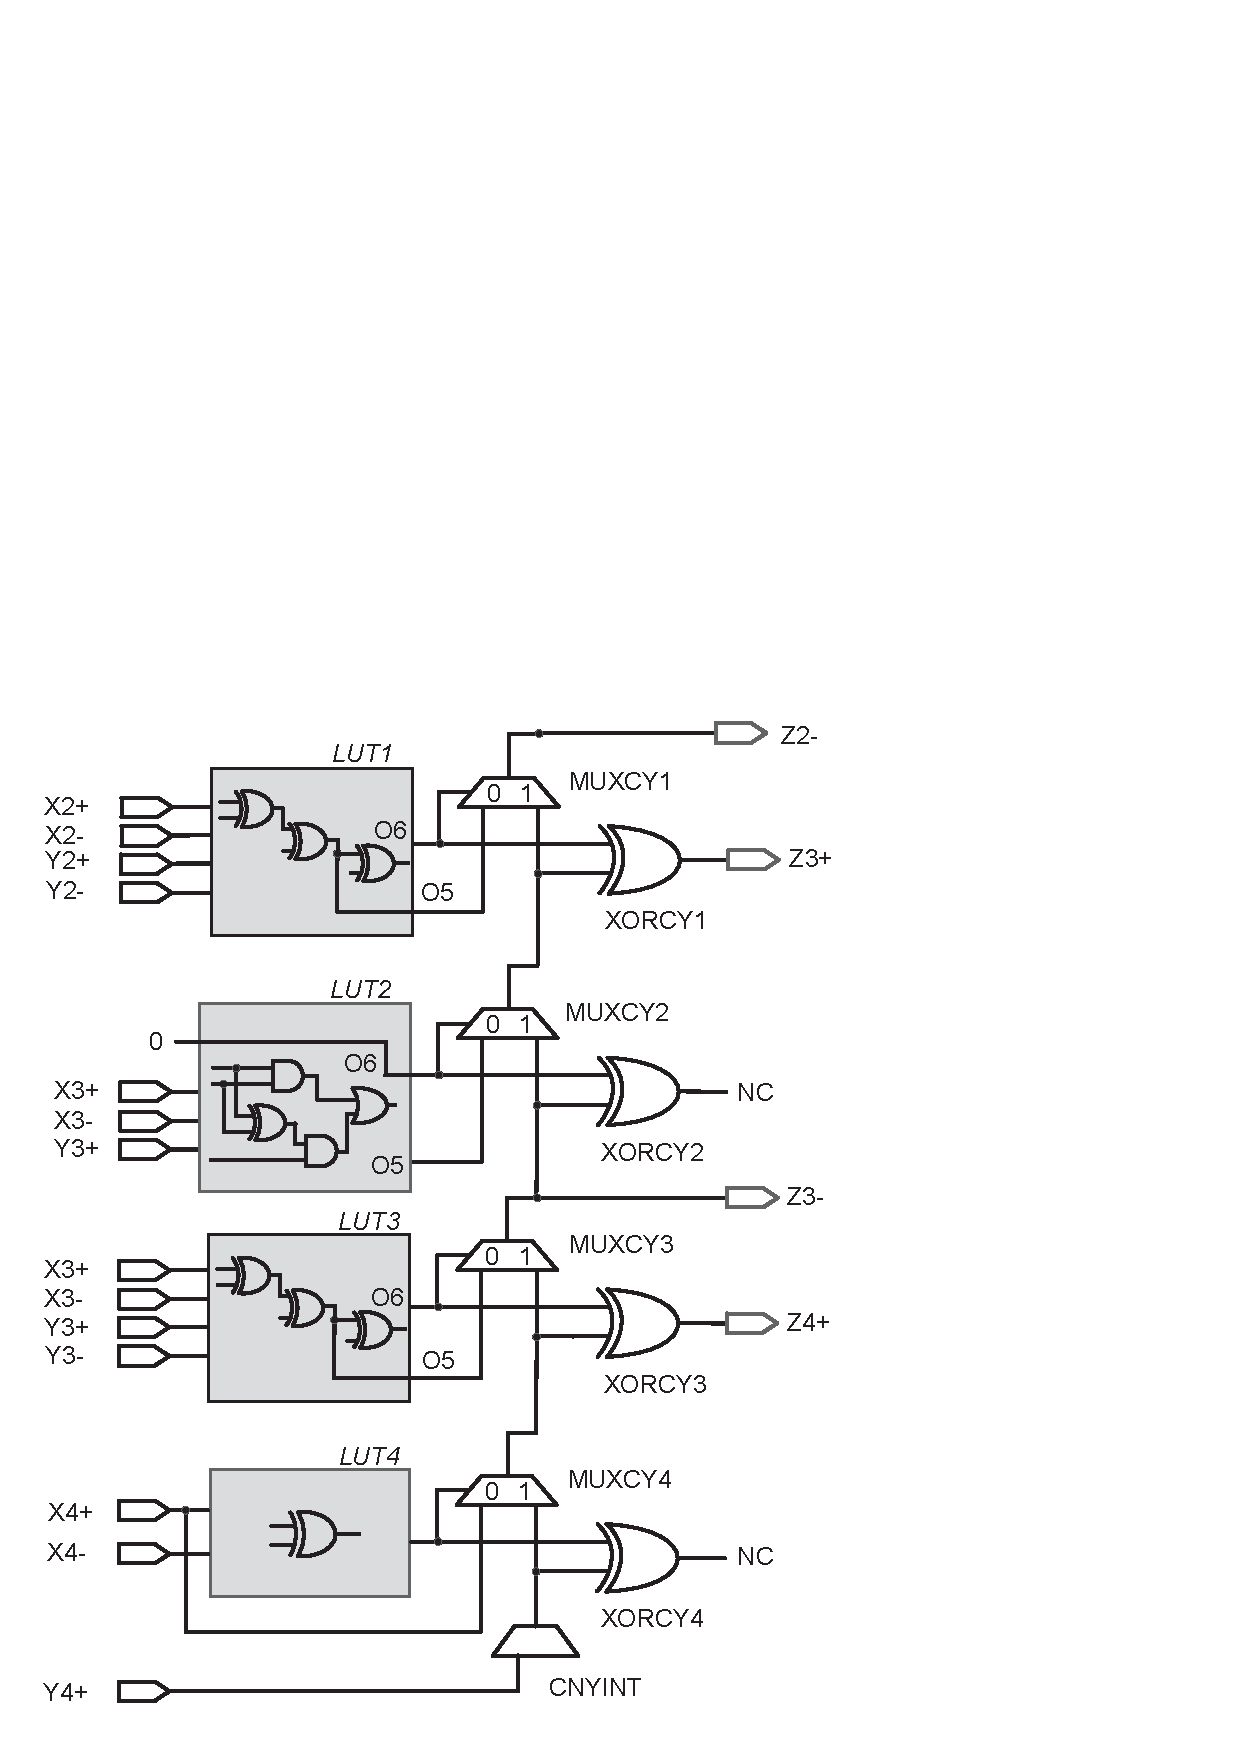
\includegraphics[width=.48\textwidth]{./Figures/SDadder_FastCarry_New.pdf}
	\caption{Implementation of 2 logic blocks (LBs) in 1 FPGA slice which contains four 6-LUTs. NC stands for Not Care.}
	\label{Fig:SliceNew}
\end{figure}

\section{Digit-parallel Online Multiplier on FPGAs}


\section{Results}



% Note that IEEE typically puts floats only at the top, even when this
% results in a large percentage of a column being occupied by floats.


% An example of a double column floating figure using two subfigures.
% (The subfig.sty package must be loaded for this to work.)
% The subfigure \label commands are set within each subfloat command, the
% \label for the overall figure must come after \caption.
% \hfil must be used as a separator to get equal spacing.
% The subfigure.sty package works much the same way, except \subfigure is
% used instead of \subfloat.
%
%\begin{figure*}[!t]
%\centerline{\subfloat[Case I]\includegraphics[width=2.5in]{subfigcase1}%
%\label{fig_first_case}}
%\hfil
%\subfloat[Case II]{\includegraphics[width=2.5in]{subfigcase2}%
%\label{fig_second_case}}}
%\caption{Simulation results}
%\label{fig_sim}
%\end{figure*}
%
% Note that often IEEE papers with subfigures do not employ subfigure
% captions (using the optional argument to \subfloat), but instead will
% reference/describe all of them (a), (b), etc., within the main caption.


% An example of a floating table. Note that, for IEEE style tables, the 
% \caption command should come BEFORE the table. Table text will default to
% \footnotesize as IEEE normally uses this smaller font for tables.
% The \label must come after \caption as always.
%
%\begin{table}[!t]
%% increase table row spacing, adjust to taste
%\renewcommand{\arraystretch}{1.3}
% if using array.sty, it might be a good idea to tweak the value of
% \extrarowheight as needed to properly center the text within the cells
%\caption{An Example of a Table}
%\label{table_example}
%\centering
%% Some packages, such as MDW tools, offer better commands for making tables
%% than the plain LaTeX2e tabular which is used here.
%\begin{tabular}{|c||c|}
%\hline
%One & Two\\
%\hline
%Three & Four\\
%\hline
%\end{tabular}
%\end{table}


% Note that IEEE does not put floats in the very first column - or typically
% anywhere on the first page for that matter. Also, in-text middle ("here")
% positioning is not used. Most IEEE journals/conferences use top floats
% exclusively. Note that, LaTeX2e, unlike IEEE journals/conferences, places
% footnotes above bottom floats. This can be corrected via the \fnbelowfloat
% command of the stfloats package.



\section{Conclusion}
The conclusion goes here.




% conference papers do not normally have an appendix


% use section* for acknowledgement
\section*{Acknowledgment}




% trigger a \newpage just before the given reference
% number - used to balance the columns on the last page
% adjust value as needed - may need to be readjusted if
% the document is modified later
%\IEEEtriggeratref{8}
% The "triggered" command can be changed if desired:
%\IEEEtriggercmd{\enlargethispage{-5in}}

% references section

\bibliographystyle{./IEEEtran}
\bibliography{./IEEEabrv,./Reference.bib}

\end{document}


